\chapter{Composite模式}
\section{组合模式的概念}
\subsection{定义}
组合(Composite)模式的定义:有时又叫作部分-整体模式,它是一种将对象组合成树状的层次结构的模式,用来表示“部分-整体”的关系,使用户对单个对象和组合对象具有一致的访问性。
\subsection{优点}
\begin{enumerate}
	\item 组合模式使得客户端代码可以一致地处理单个对象和组合对象,无须关心自己处理的是单个对象,还是组合对象,这简化了客户端代码;
	\item 更容易在组合体内加入新的对象,客户端不会因为加入了新的对象而更改源代码,满足“开闭原则”。
\end{enumerate}
\subsection{缺点}
\begin{enumerate}
	\item 设计较复杂,客户端需要花更多时间理清类之间的层次关系;
	\item 不容易限制容器中的构件;
	\item 不容易用继承的方法来增加构件的新功能。
\end{enumerate}
\subsection{模式的角色}
\begin{enumerate}
	\item Leaf树叶:表示内容的角色,角色中不能放入其他对象;
	\item Composite复合物:容器的角色,可以放入Leaf和Composite角色。
	\item Component:使得Leaf和Composite具有一致性的角色;
	\item Client:使用Composite的角色。
\end{enumerate}
\begin{figure}[!h]
	\centering
	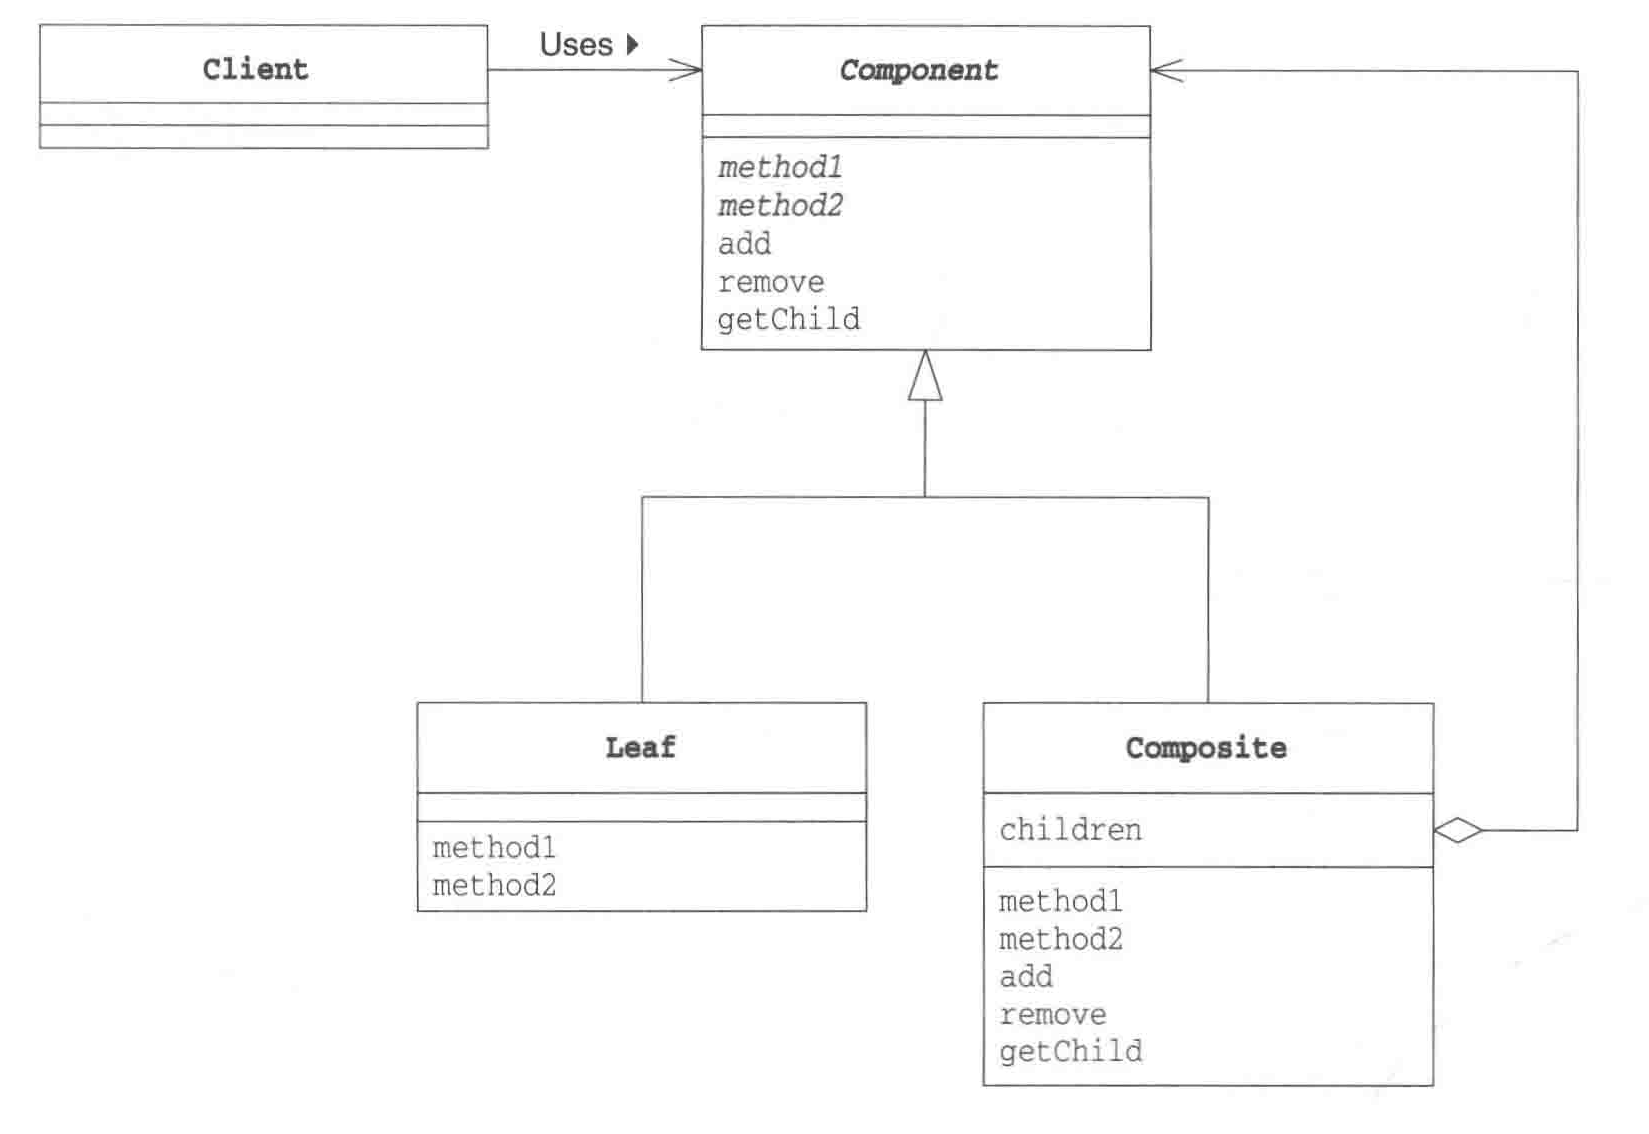
\includegraphics[width=\textwidth]{image/11-3}
	\caption{组合模式结构图}
\end{figure}
\subsection{模式的分类}
组合模式分为透明式的组合模式和安全式的组合模式。
\subsubsection{透明方式}
在该方式中,由于抽象构件声明了所有子类中的全部方法,所以客户端无须区别树叶对象和树枝对象,对客户端来说是透明的。但其缺点是:树叶构件本来没有 Add()、Remove() 及 GetChild() 方法,却要实现它们(空实现或抛异常),这样会带来一些安全性问题。
\begin{figure}[!h]
	\centering
	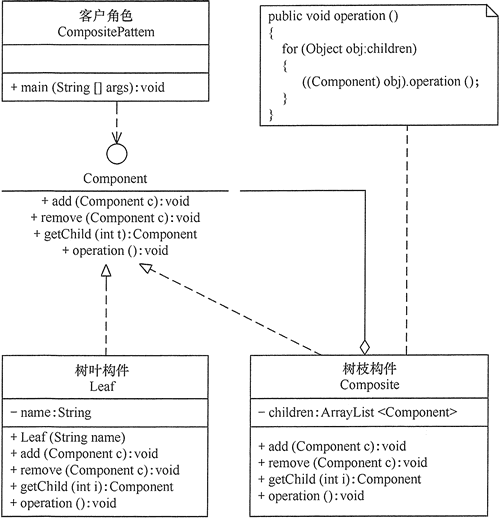
\includegraphics[width=0.8\textwidth]{image/11-1}
	\caption{透明式的组合模式的结构图}
\end{figure}
\subsubsection{安全方式}
在该方式中,将管理子构件的方法移到树枝构件中,抽象构件和树叶构件没有对子对象的管理方法,这样就避免了上一种方式的安全性问题,但由于叶子和分支有不同的接口,客户端在调用时要知道树叶对象和树枝对象的存在,所以失去了透明性。
\begin{figure}[!h]
	\centering
	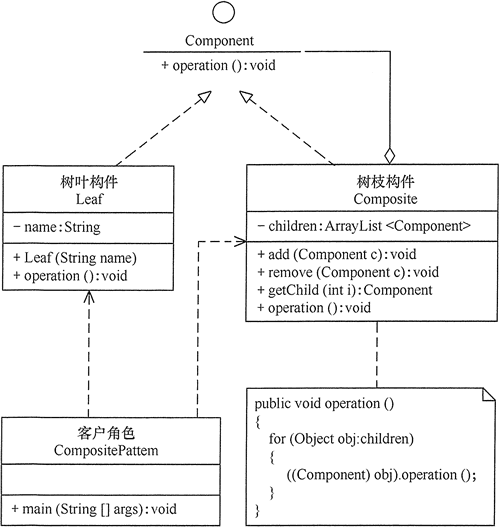
\includegraphics[width=0.8\textwidth]{image/11-2}
	\caption{安全式的组合模式的结构图}
\end{figure}
\subsection{应用场景}
\begin{enumerate}
	\item 在需要表示一个对象整体与部分的层次结构的场合;
	\item 要求对用户隐藏组合对象与单个对象的不同,用户可以用统一的接口使用组合结构中的所有对象的场合。
\end{enumerate}
\section{组合模式实现——例一}
\begin{table}[!h]
	\begin{tabular}{|l|l|}
		\hline
		名字&说明\\
		\hline
		Entry&抽象类,用来实现File和Directory的一致性\\
		\hline
		File&文件类\\
		\hline
		Directroy&文件夹类\\
		\hline
		FileTreatmentException&向文件中增加Entry是发生异常\\
		\hline
		Main&测试类\\
		\hline
	\end{tabular}
\end{table}
\begin{lstlisting}
//角色中的 Component,表示目录条目的抽象类
public abstract class Entry {
	public abstract String getName();
	public abstract int getSize();
	public Entry add(Entry entry) throws FileTreatmentException {
		throw new FileTreatmentException();
	}
	//显示目录条目一览
	public void printList() {
		printList("");
	}
	//为一览加上前缀
	protected abstract void printList(String prefix);
	
	public String toString() {
		return getName() + " (" + getSize() + ")";
	}
}
\end{lstlisting}
\begin{lstlisting}
//Leaf 角色
public class File extends Entry {
	//文件名
	private String name;
	//文件大小
	private int size;
	public File(String name, int size) {
		this.name = name;
		this.size = size;
	}
	public String getName() {
		return name;
	}
	public int getSize() {
		return size;
	}
	protected void printList(String prefix) {
		System.out.println(prefix + "/" + this);
	}
}
\end{lstlisting}
\begin{lstlisting}
// Composite 角色,表示文件夹
public class Directory extends Entry {
	//文件夹名
	private String name;
	//文件、文件夹列表
	private List<Entry> directory = new ArrayList<>();
	public Directory(String name) {
		this.name = name;
	}
	public String getName() {
		return name;
	}
	public int getSize() {
		int size = 0;
		Iterator<Entry> it = directory.iterator();
		while (it.hasNext()) {
			Entry entry = it.next();
			size += entry.getSize();
		}
		return size;
	}
	public Entry add(Entry entry) {
		directory.add(entry);
		return this;
	}
	protected void printList(String prefix) {
		System.out.println(prefix + "/" + this);
		Iterator<Entry> it = directory.iterator();
		while (it.hasNext()) {
			Entry entry = it.next();
			entry.printList(prefix + "/" + name);
		}
	}
}
\end{lstlisting}
\begin{lstlisting}
//防止对文件进行 add操作
public class FileTreatmentException extends RuntimeException {
	public FileTreatmentException() {}
	public FileTreatmentException(String msg) {
		super(msg);
	}
}
\end{lstlisting}
\begin{lstlisting}
public class Main {
	public static void main(String[] args) {
		try {
			System.out.println("Make root entries");
			Directory rootDir = new Directory("root");
			Directory binDir = new Directory("bin");
			Directory tmpDir = new Directory("tmp");
			Directory usrDir = new Directory("usr");
			rootDir.add(binDir);
			rootDir.add(tmpDir);
			rootDir.add(usrDir);
			binDir.add(new File("vi", 10000));
			binDir.add(new File("latex", 20000));
			rootDir.printList();
			
			System.out.println();
			System.out.println("Making user entries...");
			Directory yuki = new Directory("yuki");
			Directory hanako = new Directory("hanako");
			Directory tomura = new Directory("tomura");
			usrDir.add(yuki);
			usrDir.add(hanako);
			usrDir.add(tomura);
			yuki.add(new File("diary.html", 100));
			yuki.add(new File("Composite.java", 200));
			hanako.add(new File("memo.txt", 300));
			tomura.add(new File("game.doc", 400));
			tomura.add(new File("junk.doc", 500));
			rootDir.printList();
		} catch (FileTreatmentException e) {
			e.printStackTrace();
		}
	}
}
\end{lstlisting}
\section{组合模式实现——例二}
\begin{lstlisting}
//抽象构件
interface Component {
	public void add(Component c);
	public void remove(Component c);
	public Component getChild(int i);
	public void operation();
}
\end{lstlisting}
\begin{lstlisting}
//树叶构件
class Leaf implements Component {
	private String name;
	public Leaf(String name) {
		this.name = name;
	}
	public void add(Component c) {
	}
	public void remove(Component c) {
	}
	public Component getChild(int i) {
		return null;
	}
	public void operation() {
		System.out.println("树叶" + name + ":被访问!");
	}
}
\end{lstlisting}
\begin{lstlisting}
//树枝构件
class Composite implements Component {
	private ArrayList<Component> children = new ArrayList<Component>();
	public void add(Component c) {
		children.add(c);
	}
	public void remove(Component c) {
		children.remove(c);
	}
	public Component getChild(int i) {
		return children.get(i);
	}
	public void operation() {
		for (Object obj : children) {
			((Component) obj).operation();
		}
	}
}
\end{lstlisting}
\begin{lstlisting}
public class CompositePattern {
	public static void main(String[] args) {
		Component c0 = new Composite();
		Component c1 = new Composite();
		Component leaf1 = new Leaf("1");
		Component leaf2 = new Leaf("2");
		Component leaf3 = new Leaf("3");
		c0.add(leaf1);
		c0.add(c1);
		c1.add(leaf2);
		c1.add(leaf3);
		c0.operation();
	}
}
\end{lstlisting}
\begin{lstlisting}
//output
树叶1:被访问!
树叶2:被访问!
树叶3:被访问!
\end{lstlisting}
\section{模式的扩展}
如果对前面介绍的组合模式中的树叶节点和树枝节点进行抽象,也就是说树叶节点和树枝节点还有子节点,这时组合模式就扩展成\textbf{复杂组合模式}了。
\begin{figure}[!h]
	\centering
	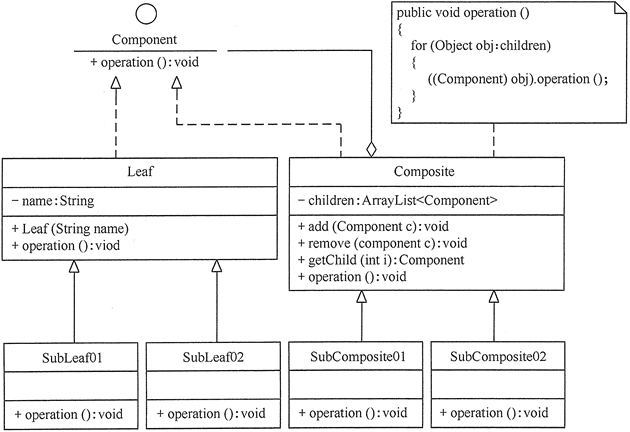
\includegraphics[width=0.8\textwidth]{image/11-4}
	\caption{复杂的组合模式的结构图}
\end{figure}
\section{扩展思路}
\begin{enumerate}
	\item 多个和单个的一致性:这里使用Composite模式使得容器和内容具有一致性;
	\item Add方法放在哪?
	\begin{enumerate}
		\item 定义在Entry类中,报错;
		\item 定义在Entry中,但什么都不做;
		\item 声明在Entry中,但不实现,但会引发安全问题;
		\item 只定义在Directory中。
	\end{enumerate}
	\item 
\end{enumerate}
\section{相关设计模式}
\begin{enumerate}
	\item Command编写宏命令使用了Composite;
	\item Vistor访问Composite中的递归结构;
	\item Decorator:Composite通过Component角色使容器和内容具有一致性。
\end{enumerate}